\section{Problem Description}\label{sec:problem_description}
By considering a free body diagram for the helicopter, such as the one in figure \textcolor{red}{INSERT}, we can derive the equations of motion as seen in equation \ref{eq:model}. Here, we assume an already implemented PID controller for the elevation, as well as an already implemented PD controller for the pitch. This leaves only the open loop travel. An explanation of the symbols used are given in table \ref{tab:model_variables}.
\begin{subequations}\label{eq:model}
	\begin{gather}
		\ddot{e} + K_{3} K_{ed} \dot{e} + K_{3} K_{ep} e = K_{3} K_{ep} e_{c}\\
		\ddot{p} + K_{1} K_{pd} \dot{p} + K_{1} K_{pp} p = K_{1} K_{pp} p_{c}\\
		\dot{\lambda} = r\\
		\dot{r} = -K_{2} p
	\end{gather}
\end{subequations}
This leads to the system seen in figure \ref{fig:layers_openloop}, which is taken from the lab assignment text.
\begin{figure}[hb]
	\centering
	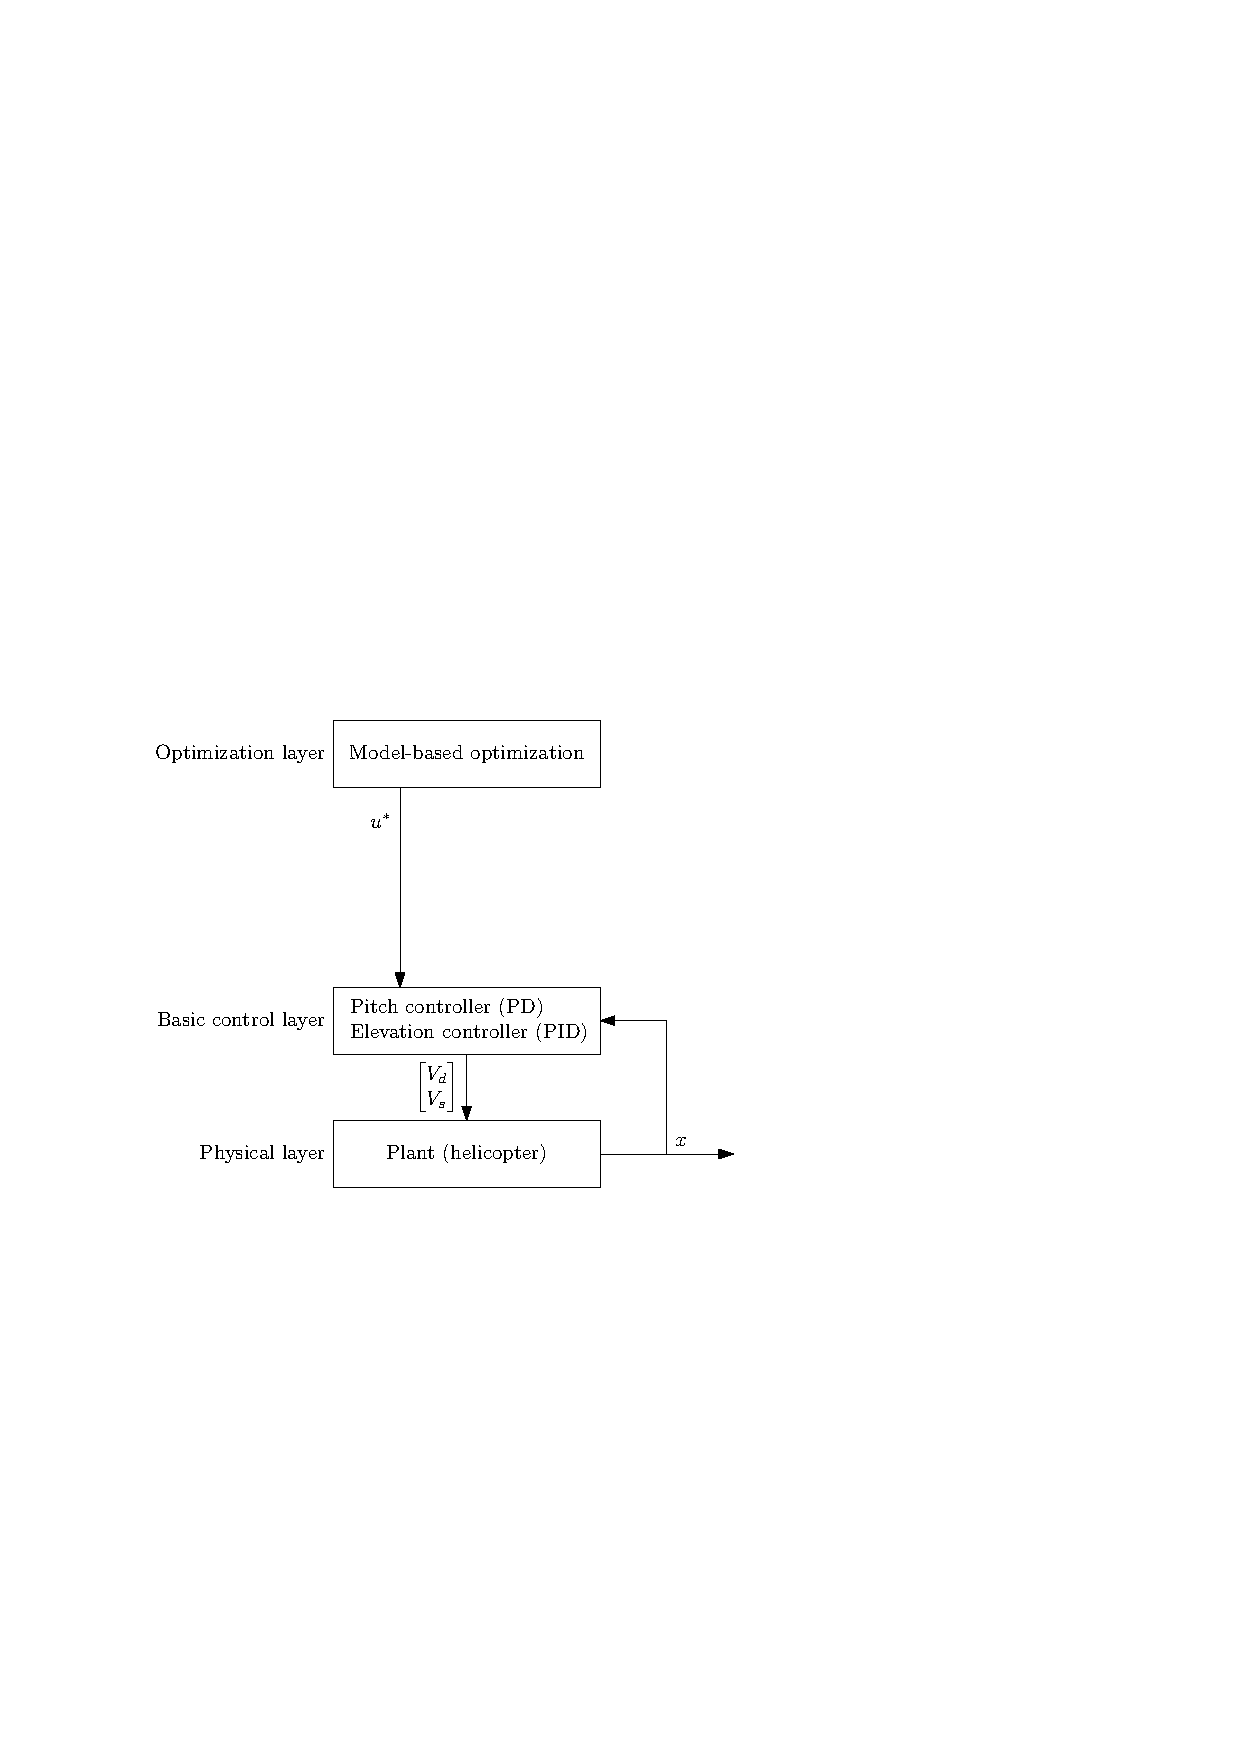
\includegraphics[width=1.00\textwidth]{figures/layers_openloop.pdf}
	\caption{Control structure under open loop travel.}
\label{fig:layers_openloop}
\end{figure}

\begin{table}[tb]
	\centering
	\caption{Variables used in equations of motion.}
	\begin{tabular}{ll}
		\toprule
		Symbol & Variable \\
		\midrule
		$p$ & Pitch\\
		$p_c$ & Pitch reference\\
		$\lambda$ & Travel\\
		$r$ & Rate of travel\\
		$r_c$ & Rate of travel reference\\
		$e$ & Elevation\\
		$e_c$ & Elevation refernce\\
		$V_f$ & Voltage, front motor\\
		$V_b$ & Voltage, back motor\\
		$V_d$ & Voltage difference, $V_f - V_b$\\
		$V_s$ & Voltage sum, $V_f + V_b$\\
		$K_{pp},\,K_{pd},\,K_{ep},\,K_{ei},\,K_{ed}$ & Controller gains\\
		$T_g$ & Momentum needed to keep helicopter in air\\
		\bottomrule
	\end{tabular}
\label{tab:model_variables}
\end{table}